\section{Evidence costs, detection and useful return}
\label{sec:post-evidence}

\subsection{Frozen study and statistical unit}

E1--E4 use $N=32768$ certification rows and a finite family of 16 queries.
The primary simultaneous level is 95\%;90\% is secondary on the same logs.
Methods share each complete log. A coverage or error observation is one
complete independent trial, never one coordinate. The six E2 outside-region
variants share a paired primitive vector within each of 300 replicate IDs;
their 1,800 condition logs are not 1,800 independent vectors. E5 contains
independent training, discovery and certification pools in each complete
trial and budgets all distinct risk and utility coordinates jointly.

For each prespecified cell/method comparison, exact one-sided binomial
undercoverage tests and Holm adjustment serve as implementation diagnostics.
Nonrejection does not prove the certificate. Wilson 95\% intervals and paired
bootstrap intervals describe Monte Carlo performance pointwise; neither is a
simultaneous statement across all displayed methods or curves. Numerical
failures and empty intervals stay in their complete-trial denominators.
Coverage, raw/intersected widths, nontriviality and decisions are reported
together. The independent-block historical study is preserved separately
in Appendix~\ref{app:post-historical}; none of its 6,000 logs was regenerated.

\subsection{Heterogeneous graphs: validity does not imply detection}

E1 crosses independent rows, a connected cycle of shared sources and a
connected chain of overlapping triangular factors with two overlap and two
outcome regimes, for 12 cells with 1,000 logs each. Conditional means vary by
row. The four policies include context dependence and are crossed with four
auditors. Exact dyadic logging lotteries and the full source-to-row incidence
define the exposure law and sufficient graph. Dependent rows retain private
sources and heterogeneous locations; they are not replicated clique records.
Bounded responses use centered Rademacher-source disturbances with absolute
coefficient sum at most .1. The heavy-tail model uses symmetric Pareto sources
with exponent 1.75 and legal $p=1.5$ envelopes from a declared location class.
The 32-bit midpoint sampler has a finite maximum and its moment envelope is
dominated by the ideal continuous-source bound; these computer samples are
not literally infinite-variance random variables.

All 96 eligible primary comparisons have complete-family coverage in
1,000/1,000 logs, with no observed false claim. The marginal Wilson 95\%
coverage interval for each fixed comparison is $[.996173,1]$.
The detection results show why this alone is insufficient. COMET detects at
least one true violation in 1,000/1,000 logs in five of six bounded cells,
but only 2/1,000 under weak overlap and triangular dependence, and 0/1,000
in every heavy-tail cell. The latter fixed-cell zero counts have marginal
Wilson upper endpoint .003827. In bounded weak-overlap independent/cycle
cells, graph Bernstein detects 1,000/1,000 whereas graph Hoeffding detects
0/1,000. The available residual range and variance budget matter substantially;
defeating the historical loose bound would not establish a new information
limit. The fully matched generic construction equals the corresponding
COMET construction.

\subsection{Local questions and irrelevant global difficulties}

E2 keeps the audited first-half mechanism fixed while changing an outside
shared-source hub size in $\{1,16,64\}$ and its exposure regime. Both local
and global queries remain in the frozen family. Global maximum-envelope and
global-coloring constructions are component ablations; local competitors
receive the same supported coefficients, nuisance, legal moments and graph.
All 60 primary comparisons cover 300/300 complete families with no observed
false claim; the fixed-comparison Wilson coverage interval is
$[.987357,1]$. COMET and the matched generic construction have zero paired
width difference in every cell, with paired-bootstrap interval $[0,0]$.
Per-query diagnostics distinguish the unchanged first-half query from global
queries whose relevant outside support actually changes. Averaging these
queries together would obscure the intended locality comparison.
For the constant-policy first-half query, the local coloring remains 2.
The pure local truncation radius is .03254654 in all six conditions, while
the bounded dispatch reduces it to .02110065. With the outside
propensity near $10^{-4}$, the global maximum-envelope radius grows from
2.2154 to 12.5324 as the outside hub grows; intersecting it with the legal
target class gives the entire class. The local interval's median
width/diameter ratio stays .04220130. Keeping local moments but paying for the
global coloring in the pure truncation engine gives normalized radii
.03255, .09206 and .18411. This comparison isolates the graph cost; the
additional reduction to .02110 is due to the eligible bounded branch.
The matched local generic baseline recovers the same protection from
irrelevant outside difficulties.

The design computation also exports 216 fixed-overlap and 216
declining-propensity configurations over sample size, subgroup mass,
exposure probability, moment order and verified coloring counts. The full
49-point production grid evaluates bias, concentration and range. These are
algebraic sufficient bounds with zero outcome draws, rather than empirical
coverage or necessary sample-size estimates.

\begin{figure}[ht]
\centering
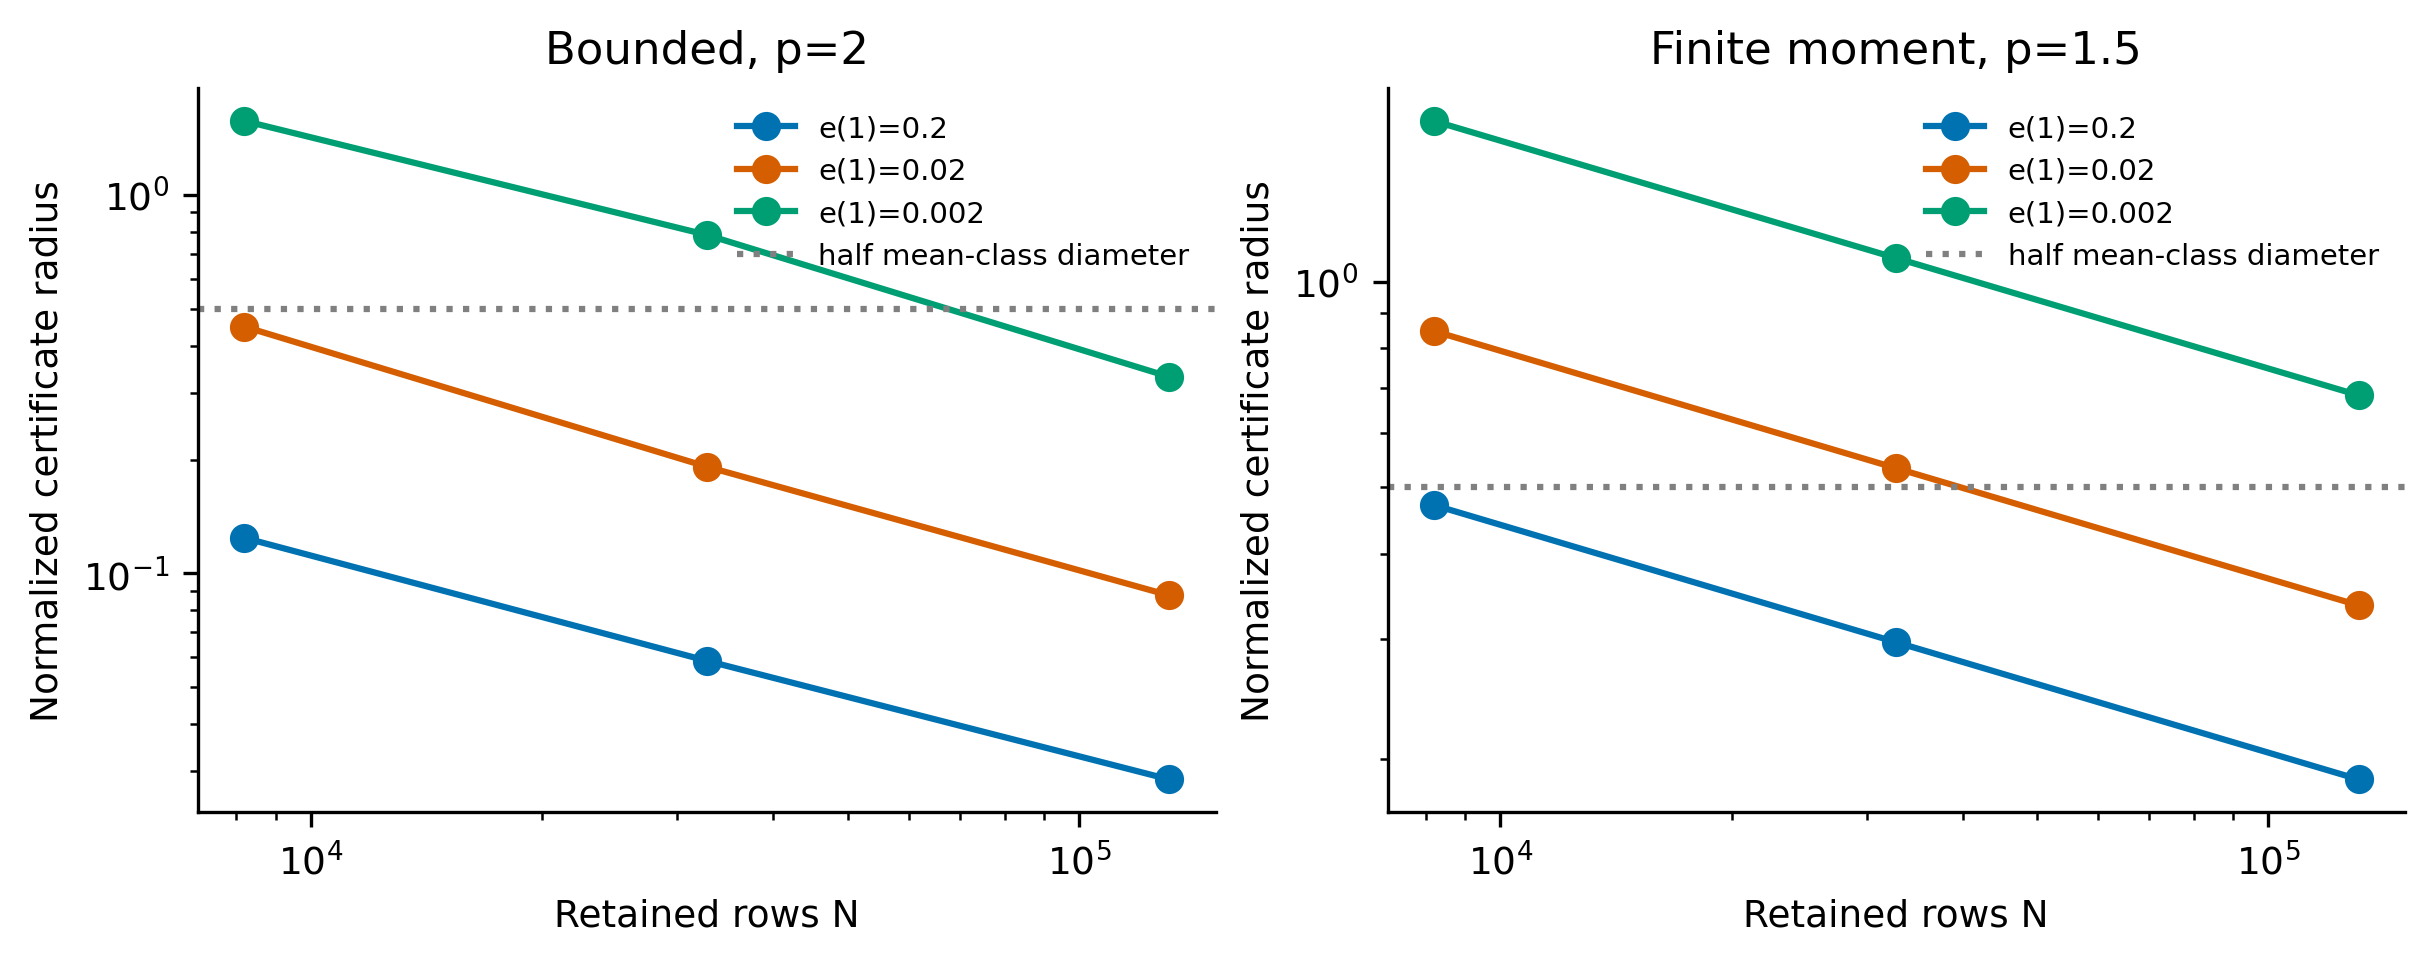
\includegraphics[width=\linewidth]{figures/design_v1/analytic_evidence_cost.png}
\caption{Deterministic normalized certificate radii at subgroup mass near .1,
available coloring count 2, family size 16 and total failure budget .05.
The bounded panel permits a design-only choice among truncation, Hoeffding
and Bernstein. The finite-moment panel uses the declared Pareto-source
residual envelope. No Monte Carlo error bars apply.}
\label{fig:post-cost}
\end{figure}

\begin{figure}[ht]
\centering
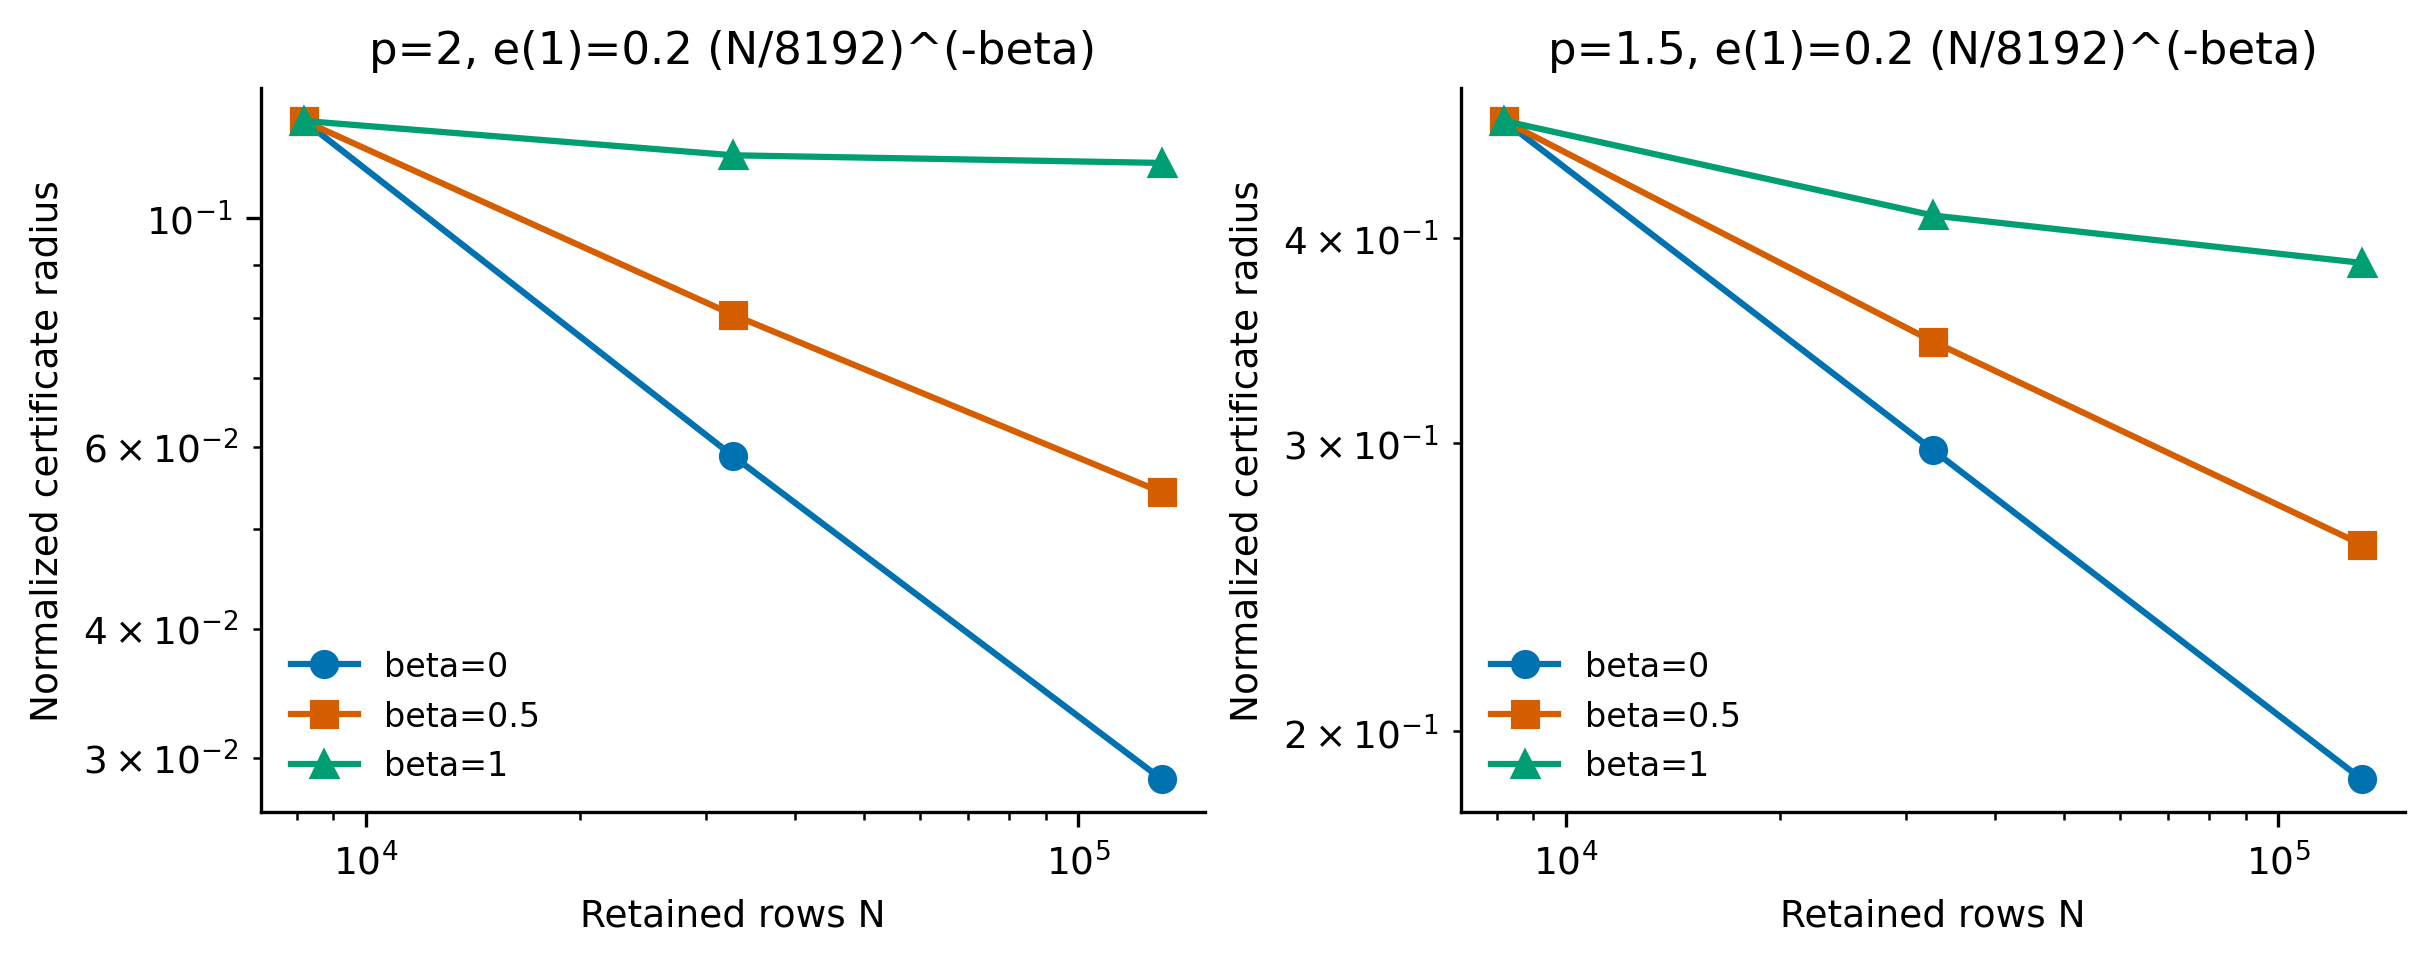
\includegraphics[width=\linewidth]{figures/design_v1/analytic_declining_overlap.png}
\caption{Declining exposure can offset growing row count. The design-only
schedule is $\epsilon_N=.2(N/8192)^{-\beta}$, with the other quantities as in
Figure~\ref{fig:post-cost}. These are procedure-specific sufficient radii,
not a sharp necessary cost or an empirical result for arbitrary weak overlap.}
\label{fig:post-declining}
\end{figure}

\subsection{Contrasts, power boundaries and the complete pipeline}

E3 compares 16 direct signed contrasts with differences of 20 distinct joint
level coordinates, including the four shared baselines only once. Both
constructions spend the same total $\delta$. Changed-support fractions are
.02,.1 and 1, crossed with the two overlap and outcome regimes. Deterministic
controls at step sizes .1,.25,.5 and 1 confirm that shrinking a signed update
scales signal and radius together. This control is not four new data sets.

All 108 primary E3 diagnostics cover 300/300 complete families, with no observed
false claim. In the full-support, moderate-overlap bounded cell, a direct
contrast certifies at least one true positive improvement in 300/300 logs;
the deduplicated joint-level difference certifies none. Mean per-trial
coordinate widths are .0066724 and .0450457 respectively under the same total
confidence budget. Every other cell has zero positive-improvement detections
for COMET, including the smaller-support cells whose raw intervals are
narrower. Thus cancellation can support a useful comparison, but a smaller
raw contrast interval alone is not evidence of higher sign-certification
power. The matched contrast-aware generic construction recovers the same
result. Noninferiority is a separate endpoint and may be easy for tiny raw
changes simply because their known feasible range is small.

E4 fixes a normalized subgroup of mass near .1, risk threshold .4 and true
gaps $\{-.10,-.03,0,.03,.10,.20\}$ in each of four environments. All 24
cells remain included. Detection, false-safe and false-violation decisions
must be interpreted alongside the known design-only $2r$ sufficient boundary;
the procedure never receives the true gap.

E5 learns nuisance functions on 4,096 training rows and discovers at most four
rules of depth at most four and minimum design mass .02 on 8,192 independent
discovery rows. At most eight policies are frozen before 32,768 certification
rows. The risk threshold is .32, utility noninferiority margin .01, service
floor .2 and capacity ceiling .6. The full deduplicated risk-plus-utility family,
typically 47 coordinates, replaces the 16-query validity family. Comparisons
include point constraints, diagnostic in-sample auditing, independent global
and local certificates, matched generic certificates, fixed slices, abstention
and uncertified status quo. The same independent-pilot candidate library is
used by proper certificate engines. Evaluation of fixed-slice and in-sample
returns uses the primary discovered constraints as well as their own-family
diagnostics.

The required pipeline endpoints are return, return and unsafe, return and
infeasible, and return and safe and useful, together with discovery and
certification of a true violation. Utility, utility gain, service, risk
violation and oracle-feasible/robust-slack comparators are evaluation-only.
Conditional unsafe-given-return is separately descriptive. Abstaining in
every trial and rejecting all service cannot count as useful success.
The incomplete E4--E5 outcomes are withheld from performance conclusions
until their fixed counts and analyses are complete.

The single selected real-covariate extension, E6 on ACS California 2018,
remains data-blocked after official-source DNS failure, HTTP403 and a browser
timeout. No E6 trial or replacement data set is reported. Its target is a
fixed-population selective-label moment, not a causal effect of selection
on income. This external limitation does not alter the synthetic protocols.
